% SPDX-License-Identifier: CC-BY-SA-4.0
%
% Copyright (C) 2026 embedded brains GmbH & Co. KG
\documentclass[tikz,border=4pt]{standalone}
\usepackage[T1]{fontenc}
\usepackage[scaled]{helvet}
\renewcommand{\familydefault}{\sfdefault}
\usetikzlibrary{arrows.meta,positioning,fit,backgrounds,calc}
\definecolor{ebblue}{HTML}{1F4E79}
\definecolor{boxfill}{HTML}{EAF1F8}
\definecolor{groupfill}{HTML}{F5F5F5}
\definecolor{flow}{HTML}{404040}
\begin{document}
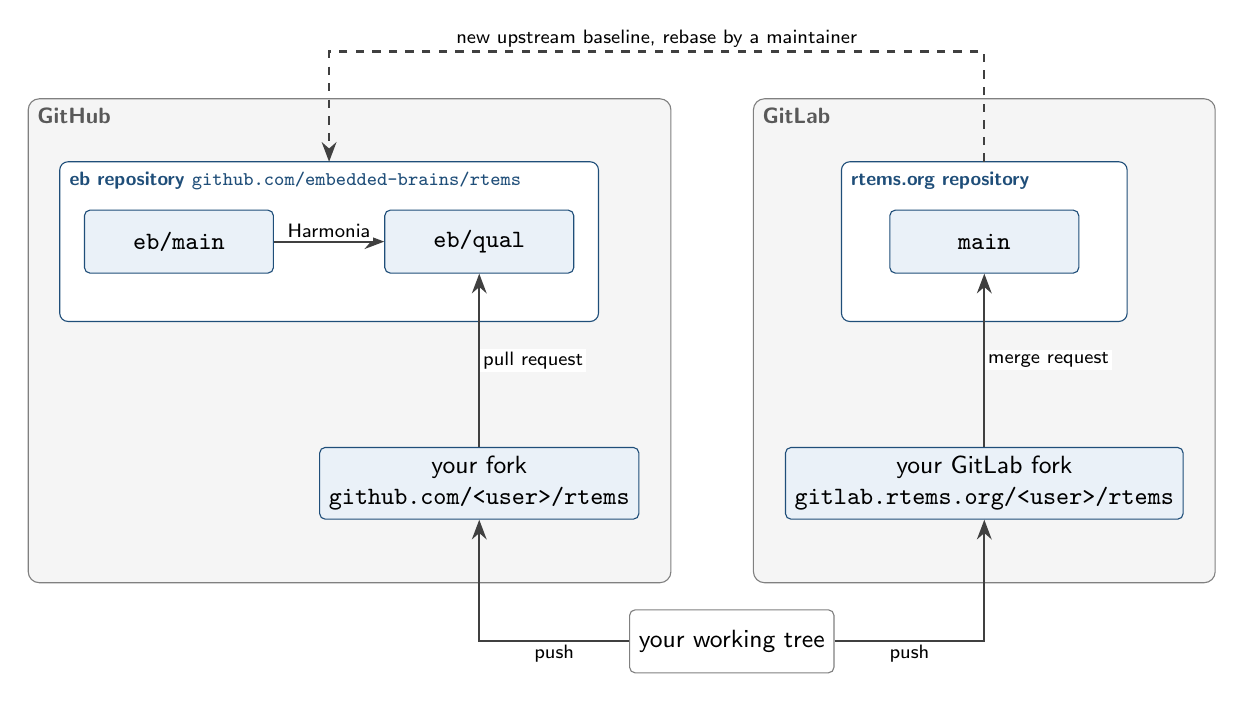
\begin{tikzpicture}[
    font=\small,
    node distance=8mm and 14mm,
    branch/.style={draw=ebblue, fill=boxfill, rounded corners=2pt,
      minimum width=24mm, minimum height=8mm, align=center},
    repo/.style={draw=ebblue, fill=white, rounded corners=3pt,
      inner sep=3mm},
    site/.style={draw=gray, fill=groupfill, rounded corners=4pt,
      inner sep=4mm},
    label/.style={font=\scriptsize\bfseries, text=ebblue},
    sitelabel/.style={font=\footnotesize\bfseries, text=gray!70!black},
    edge/.style={-{Stealth[length=2.5mm]}, thick, draw=flow},
    note/.style={font=\scriptsize, align=center, fill=white,
      inner sep=1pt}]

  % GitHub
  \node[branch] (ebmain) {\texttt{eb/main}};
  \node[branch, right=of ebmain] (ebqual) {\texttt{eb/qual}};
  \node[branch, below=22mm of ebqual] (ghfork)
    {your fork\\\texttt{github.com/<user>/rtems}};

  % GitLab
  \node[branch, right=40mm of ebqual] (rtemsorg) {\texttt{main}};
  \node[branch, below=22mm of rtemsorg] (glfork)
    {your GitLab fork\\\texttt{gitlab.rtems.org/<user>/rtems}};

  % Working tree
  \node[branch, draw=gray, fill=white,
    below=16mm of $(ghfork)!0.5!(glfork)$] (tree)
    {your working tree};

  \begin{scope}[on background layer]
    \node[repo, fit=(ebmain)(ebqual), inner ysep=6mm] (eb) {};
    \node[repo, fit=(rtemsorg), inner ysep=6mm, inner xsep=6mm] (org) {};
    \node[site, fit=(eb)(ghfork), inner ysep=8mm] (github) {};
    \node[site, fit=(org)(glfork), inner ysep=8mm] (gitlab) {};
    \fill[white, rounded corners=3pt] (eb.south west) rectangle (eb.north east);
    \fill[white, rounded corners=3pt] (org.south west) rectangle
      (org.north east);
  \end{scope}
  \draw[ebblue, rounded corners=3pt] (eb.south west) rectangle (eb.north east);
  \draw[ebblue, rounded corners=3pt] (org.south west) rectangle
    (org.north east);
  \node[label, anchor=north west] at (eb.north west)
    {eb repository \texttt{github.com/embedded-brains/rtems}};
  \node[label, anchor=north west] at (org.north west) {rtems.org repository};
  \node[sitelabel, anchor=north west] at (github.north west) {GitHub};
  \node[sitelabel, anchor=north west] at (gitlab.north west) {GitLab};

  \draw[edge] (ebmain) -- node[note, above] {Harmonia} (ebqual);
  \draw[edge] (ghfork) -- node[note, right] {pull request} (ebqual);
  \draw[edge] (glfork) -- node[note, right] {merge request} (rtemsorg);
  \draw[edge] (tree) -| node[note, pos=0.25, below] {push} (ghfork);
  \draw[edge] (tree) -| node[note, pos=0.25, below] {push} (glfork);
  \draw[edge, dashed] (org.north) |- ++(0,14mm) -| node[note, pos=0.25,
    above] {new upstream baseline, rebase by a maintainer} (eb.north);
\end{tikzpicture}
\end{document}
